\documentclass[11pt, a4paper]{article}
\usepackage{graphicx}
\usepackage{amsmath}
\usepackage{listings}
\usepackage{minted}
\usepackage{physics}
\usepackage{alltt}


\title{\underline{\textbf{\textlt{\Large{Assignment 6: The Laplace Transform}}}}}

\author{\textsl{ROHIT KUMAR [EE20B111]}}

\date{\today} 
\begin{document}	
\lstset{language=Python}
	
\maketitle % Insert the title, author and date		
  \section*{Abstract}
  The goal of this assignment are:
  \begin{itemize}
  \item
    To  explore  the  use  of  Python  libraries  in analysing Linear Time-Invariant Systems.
  \item
  	To see how RLC systems can be used as a low pass filter.
  \item
	To use the scipy signals toolkit.
  \item
	To plot blot plots to understand the Transfer function.	
\end{itemize}  	
  
  \section{Question1: Time response of a spring}
    We use Laplace transforms to solve a simple spring system.
The system is characterized by the given differential equation.(Initial conditions are zero)
\[\dv[2]{x}{t} + 2.25x = f(t) \]
and it's equivalent in Laplace domain is
\[H(s) =  \frac{1}{s^2+2.25}\]
The input signal is of the form 
\(f(t) = \cos{(\omega t)}\exp(-at)u(t)\),
where 'a' is the decay factor and $\omega$ is the frequency of the cosine signal.\\
The Laplace Transform of the input signal is
\[ F(s) = \frac{s+a}{(s+a)^2+\omega^2 }\]
We define these function these using numpy polynomials and multiply to get the output laplace transform.
Then we take the inverse laplace transform of the function using sp.impulse to get the time domain sequences and we plot these.
We do this for $\omega$=1.5, and decay of 0.5.

The python code snippet for this is shown below :-

\begin{verbatim}
Num1 = poly1d([1, 0.5])                    
Den1 = polymul([1, 1, 2.5], [1, 0, 2.25]) 
Xs_1 = sp.lti(Num1, Den1)
t1, xt_1 = sp.impulse(Xs_1, None, linspace(0, 50, 1500)) 

figure(0) # Plot of time response of the system
title("Q1: x(t) for decay of 0.5 seconds") 
xlabel("t → ", fontsize = 13)
ylabel("x(t) → ", fontsize = 13)
grid(True) 
plot(t1, xt_1)
show()

\end{verbatim}

Plot the output for an input with a decay constant of 0.5:

\begin{figure}[!tbh]
 \centering
 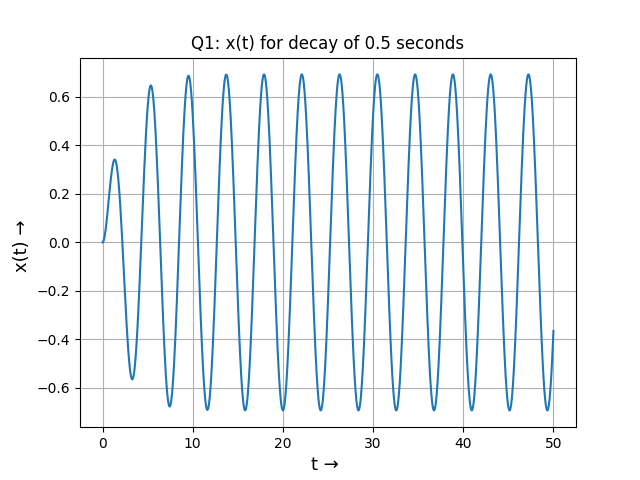
\includegraphics[scale=0.6]{Ass6_Figure_0.png}  
 \caption{Time response of a spring for decay 0.5}
\end{figure}

We observe that the output of the system in steady state is a a sinusoid with the same frequency as the input, but with no decay. 

{\textbf{This is because the natural frequency of the system is equal to the frequency of the input.}} 

  \section{Question2: Time response of spring with smaller decay(0.05)}
  The python code snippet for this is shown below :-
\begin{verbatim}
Num2 = poly1d([1, 0.05])                  
Den2 = polymul([1, 0.1, 2.2525], [1, 0, 2.25]) 
Xs_2 = sp.lti(Num2, Den2)
t2, xt_2 = sp.impulse(Xs_2, None, linspace(0, 50, 1500)) 

figure(1) # Plot of time response of the system
title("Q2: x(t) for decay of 0.05 seconds") 
xlabel("t → ", fontsize = 13)
ylabel("x(t) → ", fontsize = 13)
grid(True) 
plot(t2, xt_2)
show() 
\end{verbatim}

Plot the output for an input with a decay constant of 0.05:-  
\begin{figure}[!tbh]
 \centering
 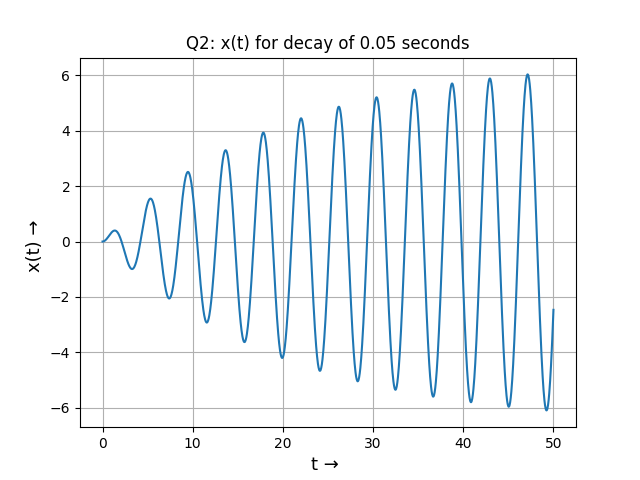
\includegraphics[scale=0.6]{Ass6_Figure_1.png}  
 \caption{Time response of a spring for decay 0.05}
\end{figure}

We observe that the steady state response follows the same trend as the previous case, except that it has a much larger amplitude.   This is because the input excited the system for a longer duration due to its smaller decay constant.   This resulted in a larger buildup of output due to resonance.  We can see that, during the buildup of the output, the amplitude grows linearly.  This is characteristic of resonance in a second order system.  This will be made clear by exciting the system with slightly different frequencies.

\section{Question3: Response over different frequencies }
To find the response to inputs with different frequencies in range of 1.4 to 1.6.

The python code snippet is shown below:-
\begin{alltt}
H = sp.lti([1], [1, 0, 2.25])
for \omega in arange(1.4, 1.6, 0.05):
	t = linspace(0, 50, 1500)
	f = cos(\omega * t) * exp(-0.05 * t)
	t3, x, svec = sp.lsim(H, f, t)


	figure(2)
	plot(t3, x, label = '\omega = ' + str(\omega))
	title("Q3: x(t) for different frequencies(\omega range from 1.4 to 1.6)")
	xlabel("t → ", fontsize = 13)
	ylabel("x(t) → ", fontsize = 13)
	legend(loc = 'upper left')
	grid(True)
show()
\end{alltt}
Plots for system responses of different frequencies are shown in a single graph:-
\begin{figure}[!tbh]
 \centering
 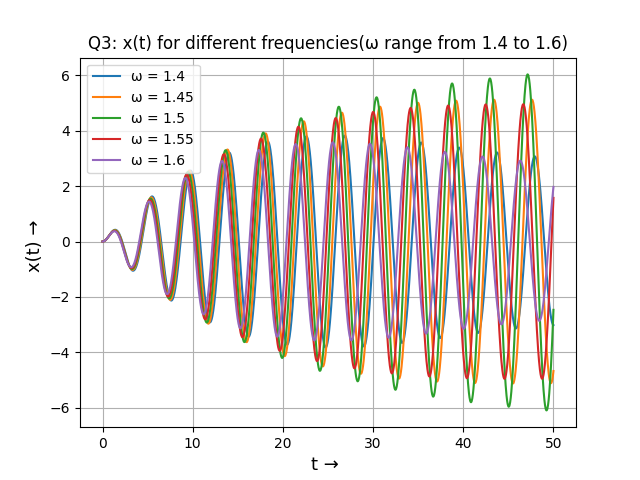
\includegraphics[scale=0.6]{Ass6_Figure_2.png}  
 \caption{System response with omega = 1.4, 1.45, 1.5, 1.55, 1.6}
\end{figure}


\cleardoublepage
We can see that the natural response of the system has the frequency $\omega$ = 1.5 rad/s. When the input frequency is at the natural frequency, the output amplitude is maximum.  In the other cases the output amplitude decreases.  This phenomenon is known as \underline{resonance}. 
\section{Question4: Coupled Spring Problem}

In this problem we have couples equations to solve for.
The equations are
\[\dv[2]{x}{t} +(x-y) = 0 \]
\[\dv[2]{y}{t} +2(y-x) = 0 \]
Given with the initial conditions
\[x(0) = 1, y(0)=\dv[1]{x(0)}{t}=\dv[1]{y(0)}{t}=0\]
We substitute for y in the second equation from the first, and we get a fourth order differential equation in terms of x.
Simplifying this and substituting to find the y equation, we get.
\[X(s) = \frac{s^2+2}{s^3+3s} \]
\[Y(s) =  \frac{2}{s^3+3s} \]
We can take the Inverse laplace Transform of these two expressions to find the time domain expressions for X(t) and Y(t).

The python code snippet for this is shown below :-
\begin{verbatim}
H4_x = sp.lti(poly1d([1, 0, 2]), poly1d([1, 0, 3, 0]))
t4, x4 = sp.impulse(H4_x, None, linspace(0, 20, 1500))
H4_y = sp.lti(poly1d([2]), poly1d([1, 0, 3, 0]))
t4, y4 = sp.impulse(H4_y, None, linspace(0, 20, 1500))  

figure(3)
plot(t4, x4, label = 'x(t)') 
plot(t4, y4, label = 'y(t)')
title("Q4: x(t) and y(t) (time responses)")
xlabel("t → ", fontsize = 13)
ylabel("Functions X(t) and Y(t) → ", fontsize = 13)
legend(loc = 'upper right')
grid(True)
show()
\end{verbatim}
The plot with X(t) and Y(t) :-
\cleardoublepage

\begin{figure}[!tbh]
 \centering
 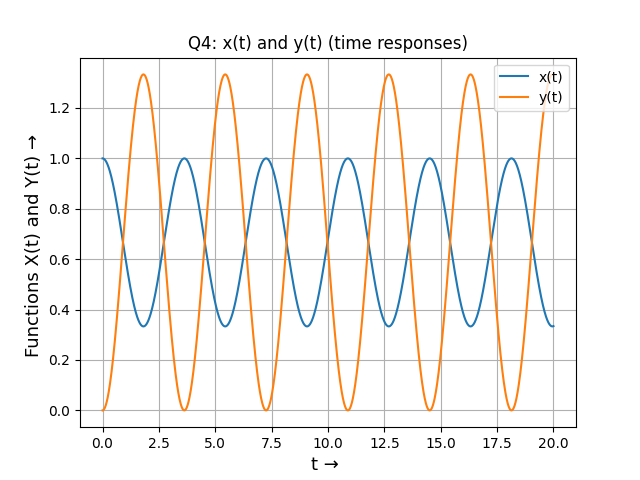
\includegraphics[scale=0.6]{Ass6_Figure_3.png}  
 \caption{The Responses of coupled system( X(t) and Y(t) )}
\end{figure}
We observe that the both X(t) and Y(t) are sinusoidal with same frequency and offsets but with different amplitude. The phase of the two are opposite.This system of equations models two masses attached to the two ends of an ideal spring with no damping. x and y are the positions of the masses in a reference frame moving at the same speed as the centre of mass, but offset from the centre of mass by some amount.

\section{Question5: RLC low pass filter}
We find the transfer function by finding the natural frequency and the damping constant of the circuit.
The RLC Filter with the transfer function as shown.
\[ H(s) = \frac{1}{10^{-12}s^2 + 10^{-4}s + 1}\]

The python code snippet is shown below :-
\begin{alltt}
\omega = 1.5 # Default Value
R = 100 
L = 1e-6 # 1e-6 <==> 10^(-6)
C = 1e-6
\omega = 1/(sqrt(L * C)) # Updating omega(ω)
Q = (1/R) * (sqrt(L/C)) # Quality factor 
\zeta = 1/(2 * Q) # Damping factor

num = poly1d([\omega**2])
den = poly1d([1, 2*\omega*\zeta, \omega**2])

H5 = sp.lti(num, den)

\omega, mag, phi = H5.bode()

# Plotting the magnitude and phase plot

figure(4) # Magnitude Plot
semilogx(\omega, mag)
title("Q5: Magnitude Bode plot")
xlabel("\omega  \rightarrow ")
ylabel("20log|H(j\omega)| \rightarrow ")
grid(True)

figure(5) # Phase plot
semilogx(\omega, phi)
title("Q5: Phase Bode plot")
xlabel("\omega  \rightarrow ")
ylabel("∠H(j\omega) \rightarrow ")
grid(True)
show()
\end{alltt}

The bode plot of the magnitude and phase response of the Steady State Transfer function of the following two-port network.

\begin{figure}[!tbh]
 \centering
 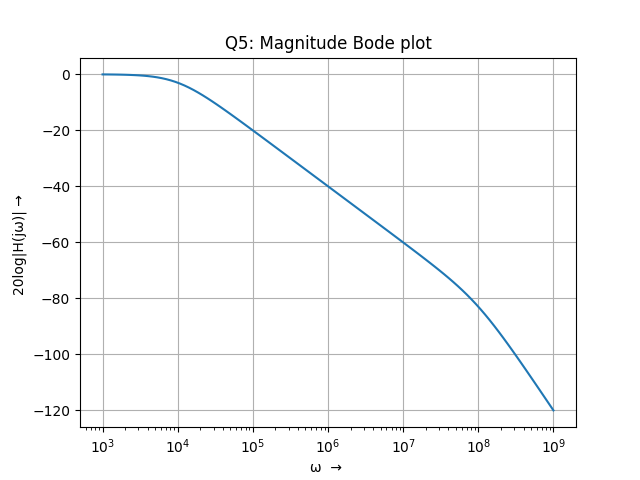
\includegraphics[scale=0.6]{Ass6_Figure_4.png}  
 \caption{The magnitude bode plot}
\end{figure}

\begin{figure}[!tbh]
 \centering
 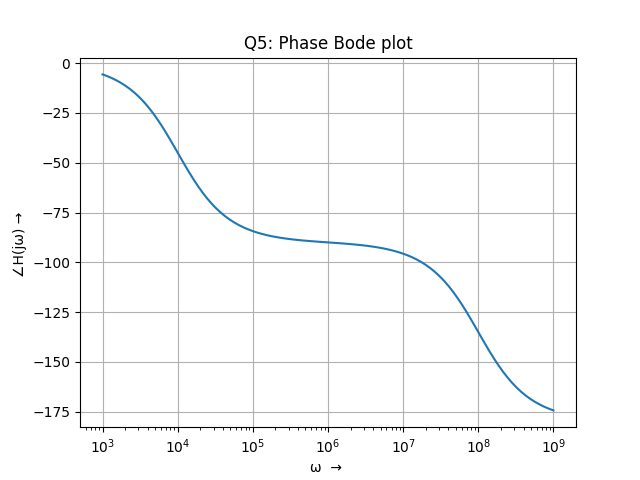
\includegraphics[scale=0.6]{Ass6_Figure_5.png}  
 \caption{The phase bode plot}
\end{figure}
\cleardoublepage

Analysis:

The system has no zeroes, it acts as an all-pole low pass filter. There are two poles, one at around $10^4$rad/s and another at around $10^8$rad/s. The system is over-damped. The 3-db bandwidth of the filter is approximately equal to $10^4$rad/sec.

\section{Question6: Obtain the output voltage v\textsubscript{0}(t) by defining the  transfer function of the system}

The input is of the form
\[x(t) = \cos{(10^3t)}-\cos{(10^6t)} \]
The output is given by
\[V\textsubscript{0}(s) =V\textsubscript{i}(s)H(s)\]


which is the superposition of two sinusoids with low and high frequencies.One whose frequency is below the 3-dB bandwith and one whose frequency is higher.
We use sp.lsim to find the output of the filter to the input system.
We plot the output from 0 to 30$\mu$s as well as from 0 to 10ms.

The python code snippet is given below :-
\begin{verbatim}
t6 = arange(0, 30e-6, 1e-8)
vi = cos(1e3 * t6) - cos(1e6 * t6)
t6, vo_short, svec = sp.lsim(H5, vi, t6)

figure(6) 
plot(t6, vo_short)
title("Q6: The Output Voltage for short time interval")
xlabel("t → ", fontsize = 13)
ylabel("v\u2092(t) → ", fontsize = 13)
grid(True)

# For Long time interval
t7 = arange(0, 10e-3, 1e-8)
vi = cos(1e3 * t7) - cos(1e6 * t7)
t7, vo_long, svec = sp.lsim(H, vi, t7)

figure(7)
plot(t7, vo_long)
title("Q6: The Output Voltage for long time interval")
xlabel("t → ", fontsize = 13)
ylabel("v\u2092(t) → ", fontsize = 13)
grid(True)
show()
\end{verbatim}
\cleardoublepage

On solving using the sp.lsim function, we get the following plot,
for 0 $<$ t $ <$30$\mu$s:

\begin{figure}[!tbh]
 \centering
 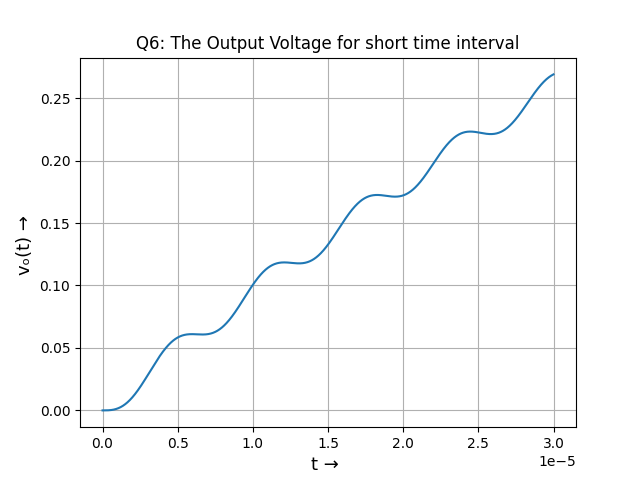
\includegraphics[scale=0.6]{Ass6_Figure_6.png} 
 \caption{The Respose for 30$mu$s}
\end{figure}
\begin{itemize}
    \item These variations are determined by the high frequency component of v(t)
\end{itemize}
\cleardoublepage
On plotting from 0 $<$ t $ <$10ms:

\begin{figure}[!tbh]
 \centering
 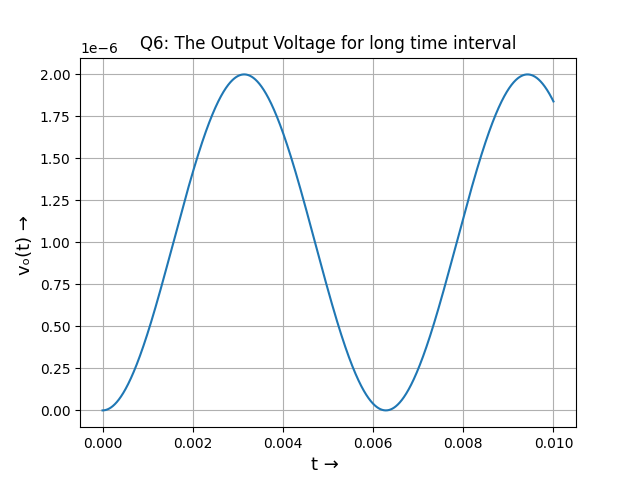
\includegraphics[scale=0.7]{Ass6_Figure_7.png} 
 \caption{The Response for 10ms}
\end{figure}
\begin{itemize}
    \item From the Bode plot,The transient response of the system is rapidly increasing.  This is because the system has to charge up to match the input amplitude.  This results in a phase difference between the input and the output.   This can also be interpreted as a delay between the input and the output signals.
    \item The high frequency component can be seen as a ripple in the short time interval plot.  This component is highly attenuated and hence not visible in the large time interval plot.
    \item In the long time interval plot, we see that the low frequency component passes almost unchanged, the amplitude is  almost  1.
    \item The  reason  is  that  the w=  $10^3$rad/s is  well  within  the  3-dB bandwidth (w3dB= $10^4$rad/s) of the system.
    \item This reiterates the fact that this is a low pass filter with bandwidth w3dB= $10^4$rad/s.
\end{itemize}

\section{ Conclusions}
\begin{itemize}
    \item The scipy.signal library provides a useful toolkit of functions for circuit analysis.The toolkit was  used for the analysis of LTI systems in various domains.
    \item The forced response of a simple spring body system was obtained over  various  frequencies  of  the  applied  force,  and  highest  amplitude  was observed at resonant frequency.
    \item The low pass filter constructed from an RLC circuit.
    \item The scipy signals acts as a toolkit to calculate the time domain response and the Bode Plot.
\end{itemize}





\end{document}